
\documentclass[11pt,a4paper]{report}%especifica o tipo de documento que tenciona escrever: carta, artigo, relatório... neste caso é um relatório
% [11pt,a4paper] Define o tamanho principal das letras do documento. caso não especifique uma delas, é assumido 10pt
% a4paper -- Define o tamanho do papel.

\usepackage[portuges]{babel}%Babel -- irá activar automaticamente as regras apropriadas de hifenização para a língua todo o
                                   %-- o texto gerado é automaticamente traduzido para Português.
                                   %  Por exemplo, “chapter” irá passar a “capítulo”, “table of contents” a “conteúdo”.
                                   % portuges -- específica para o Português.
\usepackage[utf8]{inputenc} % define o encoding usado texto fonte (input)--usual "utf8" ou "latin1

\usepackage{graphicx} %permite incluir graficos, tabelas, figuras
\usepackage{url} % para utilizar o comando \url{}
\usepackage{enumerate} %permite escolher, nas listas enumeradas, se os iems sao marcados com letras ou numeros-romanos em vez de numeracao normal

%\usepackage{apalike} % gerar biliografia no estilo 'named' (apalike)

\usepackage{color} % Para escrever em cores

\usepackage{multirow} %tabelas com multilinhas
\usepackage{array} %formatação especial de tabelas em array

\usepackage[pdftex]{hyperref} % transformar as referências internas do seu documento em hiper-ligações.

%Exemplos de fontes -- nao e vulgar mudar o tipo de fonte
%\usepackage{tgbonum} % Fonte de letra: TEX Gyre Bonum
%\usepackage{lmodern} % Fonte de letra: Latin Modern Sans Serif
%\usepackage{helvet}  % Fonte de letra: Helvetica
%\usepackage{charter} % Fonte de letra:Charter

\definecolor{saddlebrown}{rgb}{0.55, 0.27, 0.07} % para definir uma nova cor, neste caso 'saddlebrown'

\usepackage{listings}  % para utilizar blocos de texto verbatim no estilo 'listings'

\definecolor{codegreen}{rgb}{0,0.6,0}
\definecolor{codegray}{rgb}{0.5,0.5,0.5}
\definecolor{codepurple}{rgb}{0.58,0,0.82}
\definecolor{backcolour}{rgb}{0.95,0.95,0.92}

\lstdefinestyle{mystyle}{
    backgroundcolor=\color{backcolour},   
    commentstyle=\color{codegreen},
    keywordstyle=\color{magenta},
    numberstyle=\tiny\color{codegray},
    stringstyle=\color{codepurple},
    basicstyle=\ttfamily\footnotesize,
    breakatwhitespace=false,         
    breaklines=true,                 
    captionpos=b,                    
    keepspaces=true,                 
    numbers=left,                    
    numbersep=5pt,                  
    showspaces=false,                
    showstringspaces=false,
    showtabs=false,                  
    tabsize=2
}

\lstset{style=mystyle}






%paramerização mais vulgar dos blocos LISTING - GENERAL

%
%\lstset{ %
%	language=Java,							% choose the language of the code
%	basicstyle=\ttfamily\footnotesize,		% the size of the fonts that are used for the code
%	keywordstyle=\bfseries,					% set the keyword style
%	%numbers=left,							% where to put the line-numbers
%	numberstyle=\scriptsize,				% the size of the fonts that are used for the line-numbers
%	stepnumber=2,							% the step between two line-numbers. If it's 1 each line
%											% will be numbered
%	numbersep=5pt,							% how far the line-numbers are from the code
%	backgroundcolor=\color{white},			% choose the background color. You must add \usepackage{color}
%	showspaces=false,						% show spaces adding particular underscores
%	showstringspaces=false,					% underline spaces within strings
%	showtabs=false,							% show tabs within strings adding particular underscores
%	frame=none,								% adds a frame around the code
%	%abovecaptionskip=-.8em,
%	%belowcaptionskip=.7em,
%	tabsize=2,								% sets default tabsize to 2 spaces
%	captionpos=b,							% sets the caption-position to bottom
%	breaklines=true,						% sets automatic line breaking
%	breakatwhitespace=false,				% sets if automatic breaks should only happen at whitespace
%	title=\lstname,							% show the filename of files included with \lstinputlisting;
%											% also try caption instead of title
%	escapeinside={\%*}{*)},					% if you want to add a comment within your code
%	morekeywords={*,...}					% if you want to add more keywords to the set
%}

\usepackage{xspace} % deteta se a seguir a palavra tem uma palavra ou um sinal de pontuaçao se tiver uma palavra da espaço, se for um sinal de pontuaçao nao da espaço



\parindent=0pt %espaço a deixar para fazer a  indentação da primeira linha após um parágrafo
\parskip=2pt % espaço entre o parágrafo e o texto anterior

\setlength{\oddsidemargin}{-1cm} %espaço entre o texto e a margem
\setlength{\textwidth}{18cm} %Comprimento do texto na pagina
\setlength{\headsep}{-1cm} %espaço entre o texto e o cabeçalho
\setlength{\textheight}{23cm} %altura do texto na pagina

% comando '\def' usado para definir abreviatura (macros)
% o primeiro argumento é o nome do novo comando e o segundo entre chavetas é o texto original, ou sequência de controle, para que expande
\def\darius{\textsf{Darius}\xspace}
\def\antlr{\texttt{AnTLR}\xspace}
\def\pe{\emph{Publicação Eletrónica}\xspace}
\def\titulo#1{\section{#1}}    %no corpo do documento usa-se na forma '\titulo{MEU TITULO}'
\def\super#1{{\em Supervisor: #1}\\ }
\def\area#1{{\em \'{A}rea: #1}\\[0.2cm]}
\def\resumo{\underline{Resumo}:\\ }

%\input{LPgeneralDefintions} %permite ler de um ficheiro de texto externo mais definições

\title{Sistema de Gestão de Viaturas de uma Instituição\\} %Titulo do documento
%\title{Um Exemplo de Artigo em \LaTeX}
\author{João Barbosa \\(A82044) \\LCC \and João Marques\\(A84684) \\LCC \and João Reis \\(A84671) \\LCC \and Nuno Machado \\(A68702) \\LCC}
\date{\today} %data

\begin{document} % corpo do documento
\maketitle % apresentar titulo, autor e data

\begin{abstract}  % resumo do documento
Temos como principal objetivo, criar um sistema de gestão de viaturas da Instituto Politécnico de Bragança, em aplicação web de forma a otimizar todo o processo de requisição de viaturas para serviços de deslocação, substituindo toda a logística necessária em formato papel, tornando-a mais simples, intuitiva e rápida de processar. Se ainda for possível, tentaremos migrar a mesma aplicação web para uma aplicação mobile. 
\end{abstract}

\tableofcontents % Insere a tabela de indice
%\listoffigures % Insere a tabela de indice figuras
%\listoftables % Insere a tabela de indice tabelas

\chapter{Introdução} \label{chap:intro} %referência cruzada

No âmbito da unidade curricular de Projeto foi-nos proposto o desenvolvimento de uma aplicação web para um sistema de gestão de viaturas da instituição de Bragança.
Optamos pela sua construção através da linguagem \href{https://www.mysql.com/}{MySQL} para implementação da base de dados e da linguagem \href{https://www.java.com/pt-BR/download/help/whatis_java.html}{Java} para implementação das funcionalidades que necessitamos para o funcionamento de aplicação. 
Utilizamos o framework \href{https://spring.io/}{Spring} pois permite fazer a "ligação" do Back-end para o Front-end conectando-se à base de dados mencionada anteriormente. 
Iniciaremos pelo esboço do modelo conceptual de todo o projecto com as respetivas questões necessárias para o levantamento de requisitos que serão listados neste relatório. De seguida iremos assumir o modelo relacional produzindo todas as relações entre entidades/classes necessárias tendo em principal atenção o encapsulamento do mesmo.

\newpage

\chapter{Análise e Especificação} 
\section{Descrição informal do problema}
Numa instituicão existe um conjunto de viaturas (com ou sem motorista) que podem ser requisitadas para um determinado serviço de deslocação. A ideia seria desenvolver uma aplicação web que permitisse efectuar um pedido de viatura para um determinado serviço (capacidade da viatura, dia de ida, dia de vinda, horas, local de destino).
Esse pedido terá que ser validado em termos de disponibilidade pela própria aplicação atribuindo uma viatura ao serviço e, em termos de autorização, por parte de uma entidade superior. Caso o pedido seja aceite é inserido no calendário de requisições autorizadas. O sistema poderá ser otimizado com sugestões de boleias partilhadas (total ou parcialmente), com alternativas de viaturas com menor capacidade ou com horas próximas que permitiriam a requisição da viatura.
\label{sec:descricaoProblema} %seccao e referencia cruzada
\newpage
\section{Especificação dos Requisitos}
Após definidos os objetivos da nossa aplicação estabelecidos pela cliente, percebemos que teríamos essencialmente de priorizar a organização da aplicação guardando assim vários registos. Assim sendo fomos capazes de identificar os seguintes requisitos: \newline

\begin{enumerate}[]
\item \textbf{\underline {Veículo}}: a nossa aplicação terá vários veículos que serão reservados para a realização de viagens solicitados pelo utilizador. Existirão vários veículos registados distinguidos essencialmente pela sua matrícula onde serão gravadas várias características, sendo elas, a marca, o modelo, os quilómetros, o ano, a cor, os lugares, e o seu combustível. Esse veículo poderá ou não ter motorista atribuído e será possível verificar se está em utilização.

\item \textbf{\underline {Utilizador}}: a nossa aplicação será gerida para um utilizador que terá a possibilidade de fazer reservas de veículos para fazer deslocações (viagem). Será identificado pelo id, tendo ainda como características o seu nome e apelido, e ainda um código.

\item \textbf{\underline {Viagem}}: a principal "mecânica" da nossa app serve em grande parte para facilitar as deslocações. Essas deslocações que serão feitas através de veículos reservados pelos utilizadores serão identificadas pelo seu id, tendo como características o local de inicio, o local do fim, os kms iniciais, os kms finais, a hora de inicio e hora de fim, o nº de passageiros, e o seu motivo.

\item \textbf{\underline {Gestor}}: Será a entidade responsável pela gestão dos veículos, será capaz de adicionar ou remover um veículo da app.

\item \textbf{\underline {Secretaria}}: Será a entidade responsável pela confirmação e/ou validação das viagens solicitadas. 



\end{enumerate}
\newpage
\subsection{Entrevista à Cliente}

\textbf{1. Que informacoes é necessario manter sobre cada veiculo?}

R: matricula, nº de lugares, escola a que pertence, marca, submarca, anos de vida, cor, tipo de combustível, tipo de carro (ver abaixo), com ou sem motorista.
\newline
\textbf{2. E necessario criar um perfil de cada pessoa? Se sim, que informações deveriamos guardar sobre cada pessoa que reserva um carro?}

R: o utilizador deve ser validado por LDAP, ou seja, deve usar o login da instituicao a que pertence e ao fazer a requisicao fica associado ao seu login.
Mas isso pode ser visto depois. Neste momento devemos associar a cada requisicao apenas o nome e nº de funcionario que esta a fazer a requisicao.
\newline
\textbf{3. Que informacoes é necessario obter ao final de cada viagem e ao inicio de cada viagem?}

R: hora de inicio, local de inicio, nº de quilometros iniciais do carro, nº e nome de passageiros hora fim, local de fim, nº quilometros finais do carro.
\newline
\textbf{4. Que informacoes deveriamos ter sobre cada viagem?}

R: Para alem do destino, data e hora talvez o objectivo da viagem e para alem do que esta na questao anterior adicionar no final da viagem o feedback sobre o estado do carro ou de alguma ocorrencia a registar
\newline
\textbf{5. Como e que podemos diferenciar os diferentes veiculos?}

R: matricula
tipo de carro: carro, jipe, autocarro, carrinha, etc
\newline
\textbf{6. Sobre cada viagem, que informacao e que precisamos ter?  Devemos manter o perfil da pessoa que reserva o veiculo para esse utilizador ir informando quantos lugares estao disponiveis?}

R: ao fazer a requisicao indicar o nome e nº de passageiros, no inicio da viagem confirmar os passageiros
\newline
\textbf{7. Que restricoes uma certa pessoa que queira reservar um veiculo para uma certa viagem pode ter? (Restricoes de horario, restricoes relativas a uma certa autorizacao necessaria) Só docentes podem reservar veiculos ou alunos tambem podem? Que diferenciacao havera entre diferentes docentes e funcionarios da instituicao}

R: Os alunos nao podem reservar viaturas, apenas os funcionarios (docentes ou nao-docentes) o poderao fazer e isso vai ter que ser validado de alguma forma.
\newline
\textbf{8. Como e que uma pessoa que queira juntar-se a uma certa viagem deve informar a pessoa que esta encarregue dessa viagem? deve ser guardado o meio de contacto da pessoa responsavel pela viagem e os passageiros interessadas na viagem devem entrar em contacto com essa pessoa?}

R: SIM, deve entrar em contacto com a pessoa que requisitou o carro e se se consumar a boleia essa pessoa deve ser inserida pelo condutor como passageiro.
\newline
\textbf{8.1. A pessoa que reserva a viagem fica responsavel de quem vai na viagem? Ou simplesmente a pessoa que reserva o veiculo para a certa viagem apenas fica responsavel pelo carro durante a viagem e as pessoas que se queiram juntar simplesmente "adicionam-se"}

\textbf{9. Caso o veiculo seja utilizado numa visita de estudo, que propriedades são interessantes registar que as diferem de uma viagem normal}
  
R: nada
\newline
\textbf{10. Quando se seleciona um horario de reserva de um veiculo, podem acontecer imprevistos que não possiblitem a utilizacao do automovel nos horarios que seguem, como um atraso. A aplicacao deve ser capaz de avisar ao utilizador seguinte que o horario que selecionou nao tem veiculos disponiveis?}

R: Quando o condutor anterior sinalizar um atraso o condutor seguinte devia ser notificado.
\newpage
\textbf{11. Dada uma viagem concluida, a aplicação deve ser capaz de marcar um veiculo como livre para outra viagem?}

R: Sim, condutor no final da viagem deve fazer o checkout.
\newline
\textbf{12. No evento de um acidente como devemos processar a informacao?}

R: no feedback final do condutor deve ficar registado o acidente
\newline
\textbf{13. No evento de um acidente como é que a pessoa responsavel pela viagem e pelo veiculo devem atuar e quem e que devem avisar? Eles tem que avisar no momento do acidente e seriam informados de como proceder?} 

R: Como qualquer condutor ...
\newline
\textbf{14. Quem fica responsavel pelas chaves dos veiculos ou pelo armazenamento dos veiculos na universidade?}

R: A portaria
\newline
\textbf{15. A aplicacao devera manter registo da condicao mecanica dos diferentes veiculos?}

R: Os documentos de revisao do carro estão dentro do carro.
A aplicação apenas servira para notificar necessidades de manutencao
\newline
\textbf{16. Ha motoristas para autocarros que devam ser adicionados ao sistema?}

R: Ha veiculos com motorista e veiculos sem motorista. Ambos são passiveis de requisicao.
\newline
\textbf{17. Como e que os gestores dos veiculos na universidade atuam no caso de certos veiculos necessitarem de manutencao? Todos os veiculos vao para a mesma oficina? Ou criam um registo apenas para saberem que esse veiculo foi para manutencao para uma certa oficina e saberem qual oficina?}

R: Nao e necessario gerir essa informacao.
\newline
\textbf{18. Como podemos diferenciar as pessoas que utilizam este serviço?}

R: Pelo nº de funcionario
\newline
\textbf{19. A aplicação fica responsavel pela lotacao do veiculo?}

R: Cada veiculo tem uma lotacao que nao pode ser excedida. A aplicacao nao deve deixar introduzir um nº de passageiros superior a lotacao do veiculo.
\newline
\textbf{20. Devera haver veiculos disponiveis imediatamente no caso de uma emergencia?
Veiculos estes que não necessitem de reservar uma hora para viagem.}

R: Nao. Esses nao entram na aplicação
\newline
\textbf{21. Que mais informacao sera guardada momento da reserva do veiculo para alem de horario de reserva, veiculo em questão, nome do condutor, etc?}

R: Nº de funcionario requisitante, tipo de carro, nº de passageiros, local de destino, data e hora prevista de saida e chegada, motorista?, motivo da requisicao.
\newline
\textbf{22. O portal de registo da aplicacao deve ser acessivel pela internet?}

R: Sim
\newline
\textbf{23. Devemos encriptar os credenciais dos utilizadores da aplicacao?}

R: Deviamos usar o sistema de autenticacao LDAP
\newline
\textbf{24. Quem e que determina se as propostas de viagens são viaveis ou nao para serem aceites para a reserva de um certo veiculo? Existe algum moderador para a autorizacao do certo veiculo para a certa viagem?}

R: Talvez um elemento da direcao da escola ou da secretaria.
\newline
\textbf{25. Deve haver diferentes tipos de gestores com diferentes responsabilidades?}

R: Vamos tentar nao complicar muito a este respeito. Talvez apenas um tipo de gestor que gere a informacao dos veiculos e valida as requisições
\newpage
\textbf{26. Na reserva de um veiculo, a pessoa pode selecionar um a escolha, ou e-lhe atribuido um veiculo?}

R: Pode selecionar dentro dos disponiveis.
\newline
\subsection{Levantamento dos Requisitos}

\begin{enumerate}

\item Devemos manter, de cada veículo, a matricula, número de lugares, escola a que pertence, marca, submarca, anos de vida, cor, tipo de combustível, tipo de carro, com ou sem motorista.

\item Devemos associar a cada requisição apenas o nome e número de funcionário que está a fazer a requisição

\item Ao inicio de cada viagem devemos obter, a hora de inicio, local de inicio, nº de quilometros iniciais do carro e o número de passageiros

\item Ao final de cada viagem devemos obter, a hora do fim, local do fim e o número de quilometros finais do carro

\item Para além do que obtemos no ínicio e final de viagem, devemos obter também, o destino, data, objetivo da viagem e o feedback sobre o estado do carro ou de alguma ocorrência a registar

\item Devemos diferenciar os diferentes veículos pela matricula e pelo tipo de carro: carro, jipe, autocarro, carrinha, etc.

\item No inicio de cada viagem devemos confirmar o id dos passageiros a bordo do veículo

\item Um condutor deve ter a opção de adicionar outros utilizadores a uma reserva

\item Deve ser capaz de notificar o usuário sobre um atraso na disponibilidade do veiculo

\item Dada uma viagem concluida, deve ser capaz de marcar um veiculo como livre para outra viagem, atravez de uma funcionalidade de checkout

\item O condutor deve poder registar um acidente

\item Deve informar sobre a necessidades de manutenção de um veículo

\item Deve poder registar veículos com e sem motorista

\item Cada utilizador deve ter um ID de funcionário

\item Cada veiculo tem uma lotação que não pode ser excedida.

\item Os veículos, para casos de emergência, são tratados à parte e por isso não se mantêm registo sobre eles.

\item No momento de fazer a reserva, são mantidas a matrícula do veículo em questão, nº de funcionário requisitante, o tipo do carro em questão, o nº previsto de passageiros, o local de Destino, a data e hora previstas de saída, a data e hora previstas de chegada e o motivo da requisição.

\item O portal de registo da aplicação deve ser acessível pela internet.

\item Os utilizadores da aplicação são aceites pelo sistema de autenticação LDAP.

\item A secretaria é responsável pela validação das propostas de reserva.

\item Deve haver um gestor que gere as informações dos veículos

\item O condutor deve poder selecionar entre veículos disponíveis
 
\item Apenas funcionários da universidade podem reservar viagens
\end{enumerate}




%\VerbatimInput{teste1.txt}



\newpage

\chapter{Concepção/desenho da Resolução}

\section{Modelo Conceptual}
\begin{figure}[h!]
\centering
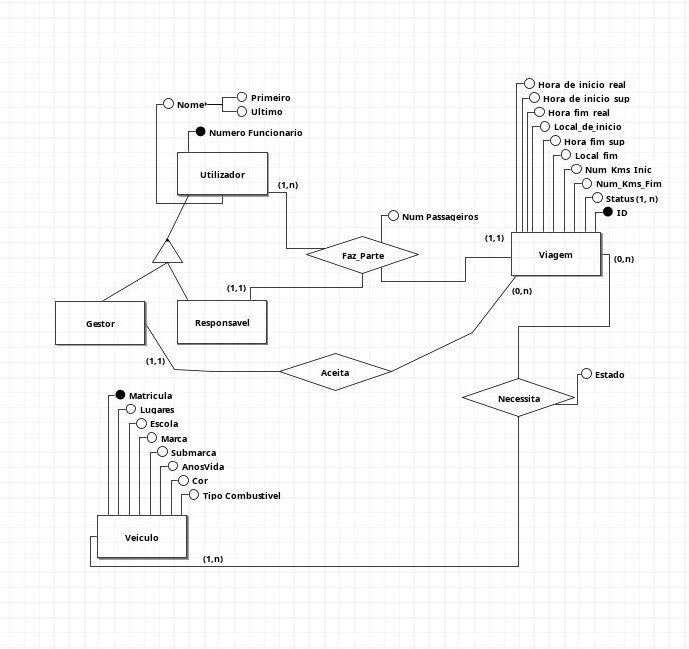
\includegraphics[scale=0.5]{Pictures/diagrama.jpg}
\caption{\label{fig:html} Modelo Conceptual da aplicação}
\end{figure}
\newpage
\section{Diagrama UseCase}

\begin{figure}[h!]
\centering
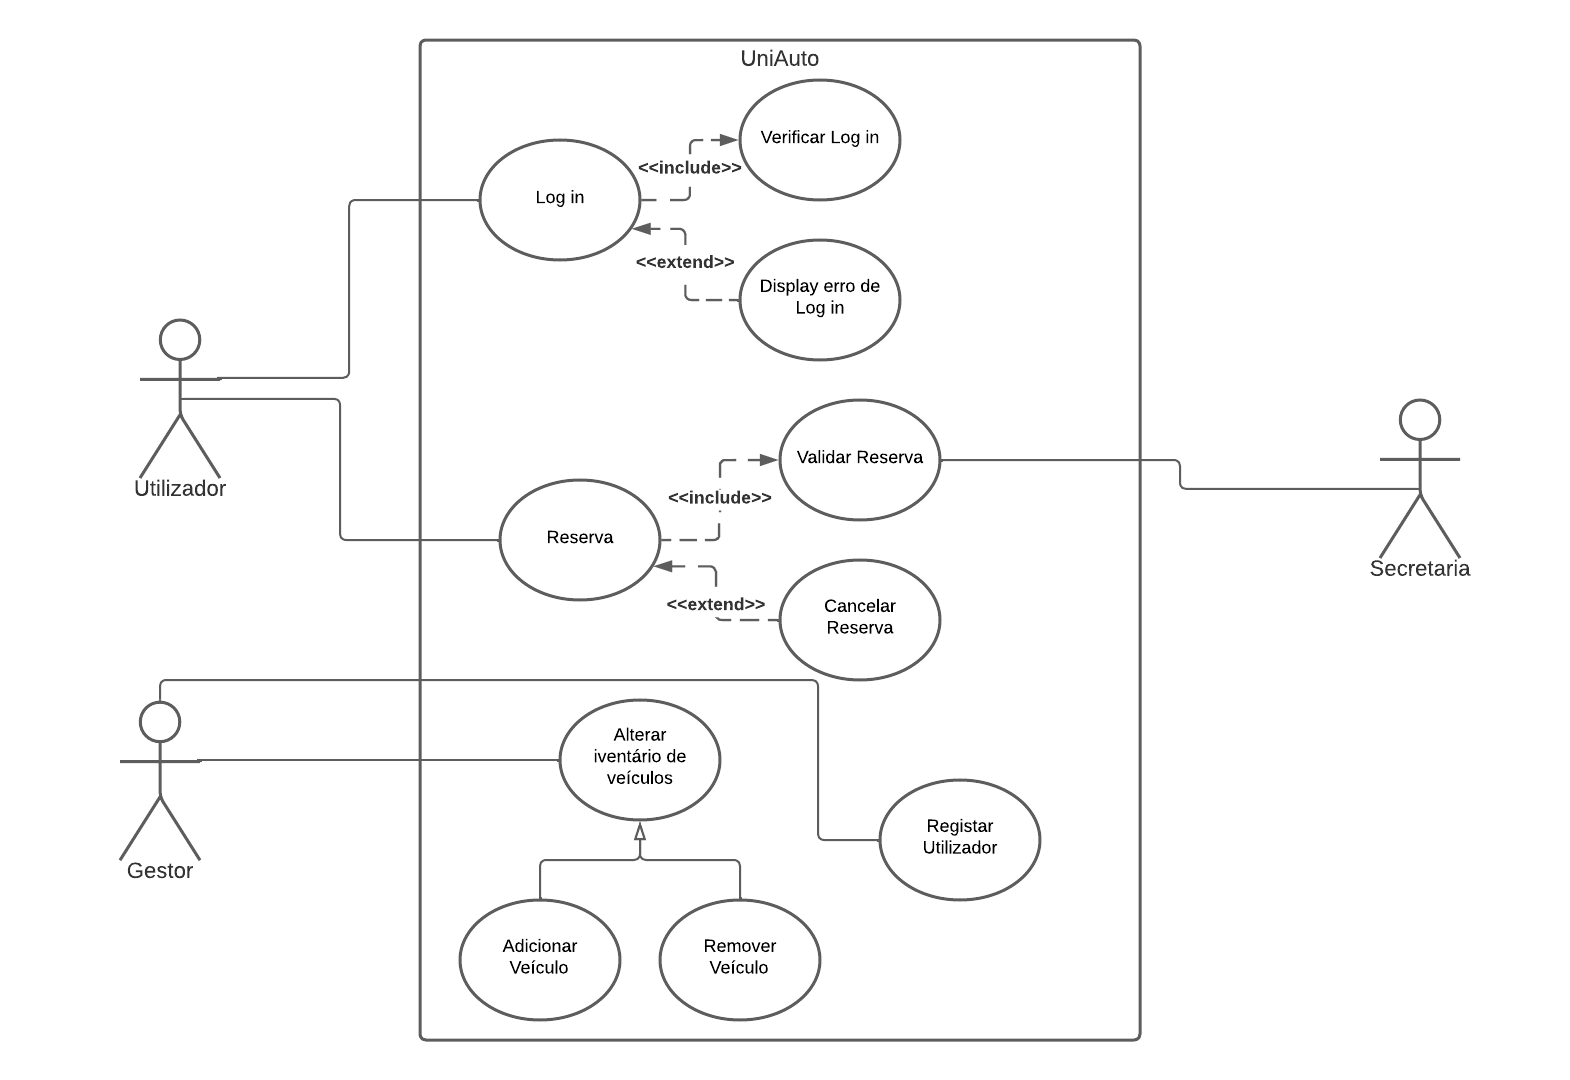
\includegraphics[scale=0.6]{Pictures/UniAuto.png}
\caption{\label{fig:Diagrama} Diagrama UseCase}
\end{figure}
\newpage
\section{Diagrame de Classes}
\begin{figure}[h!]
\centering
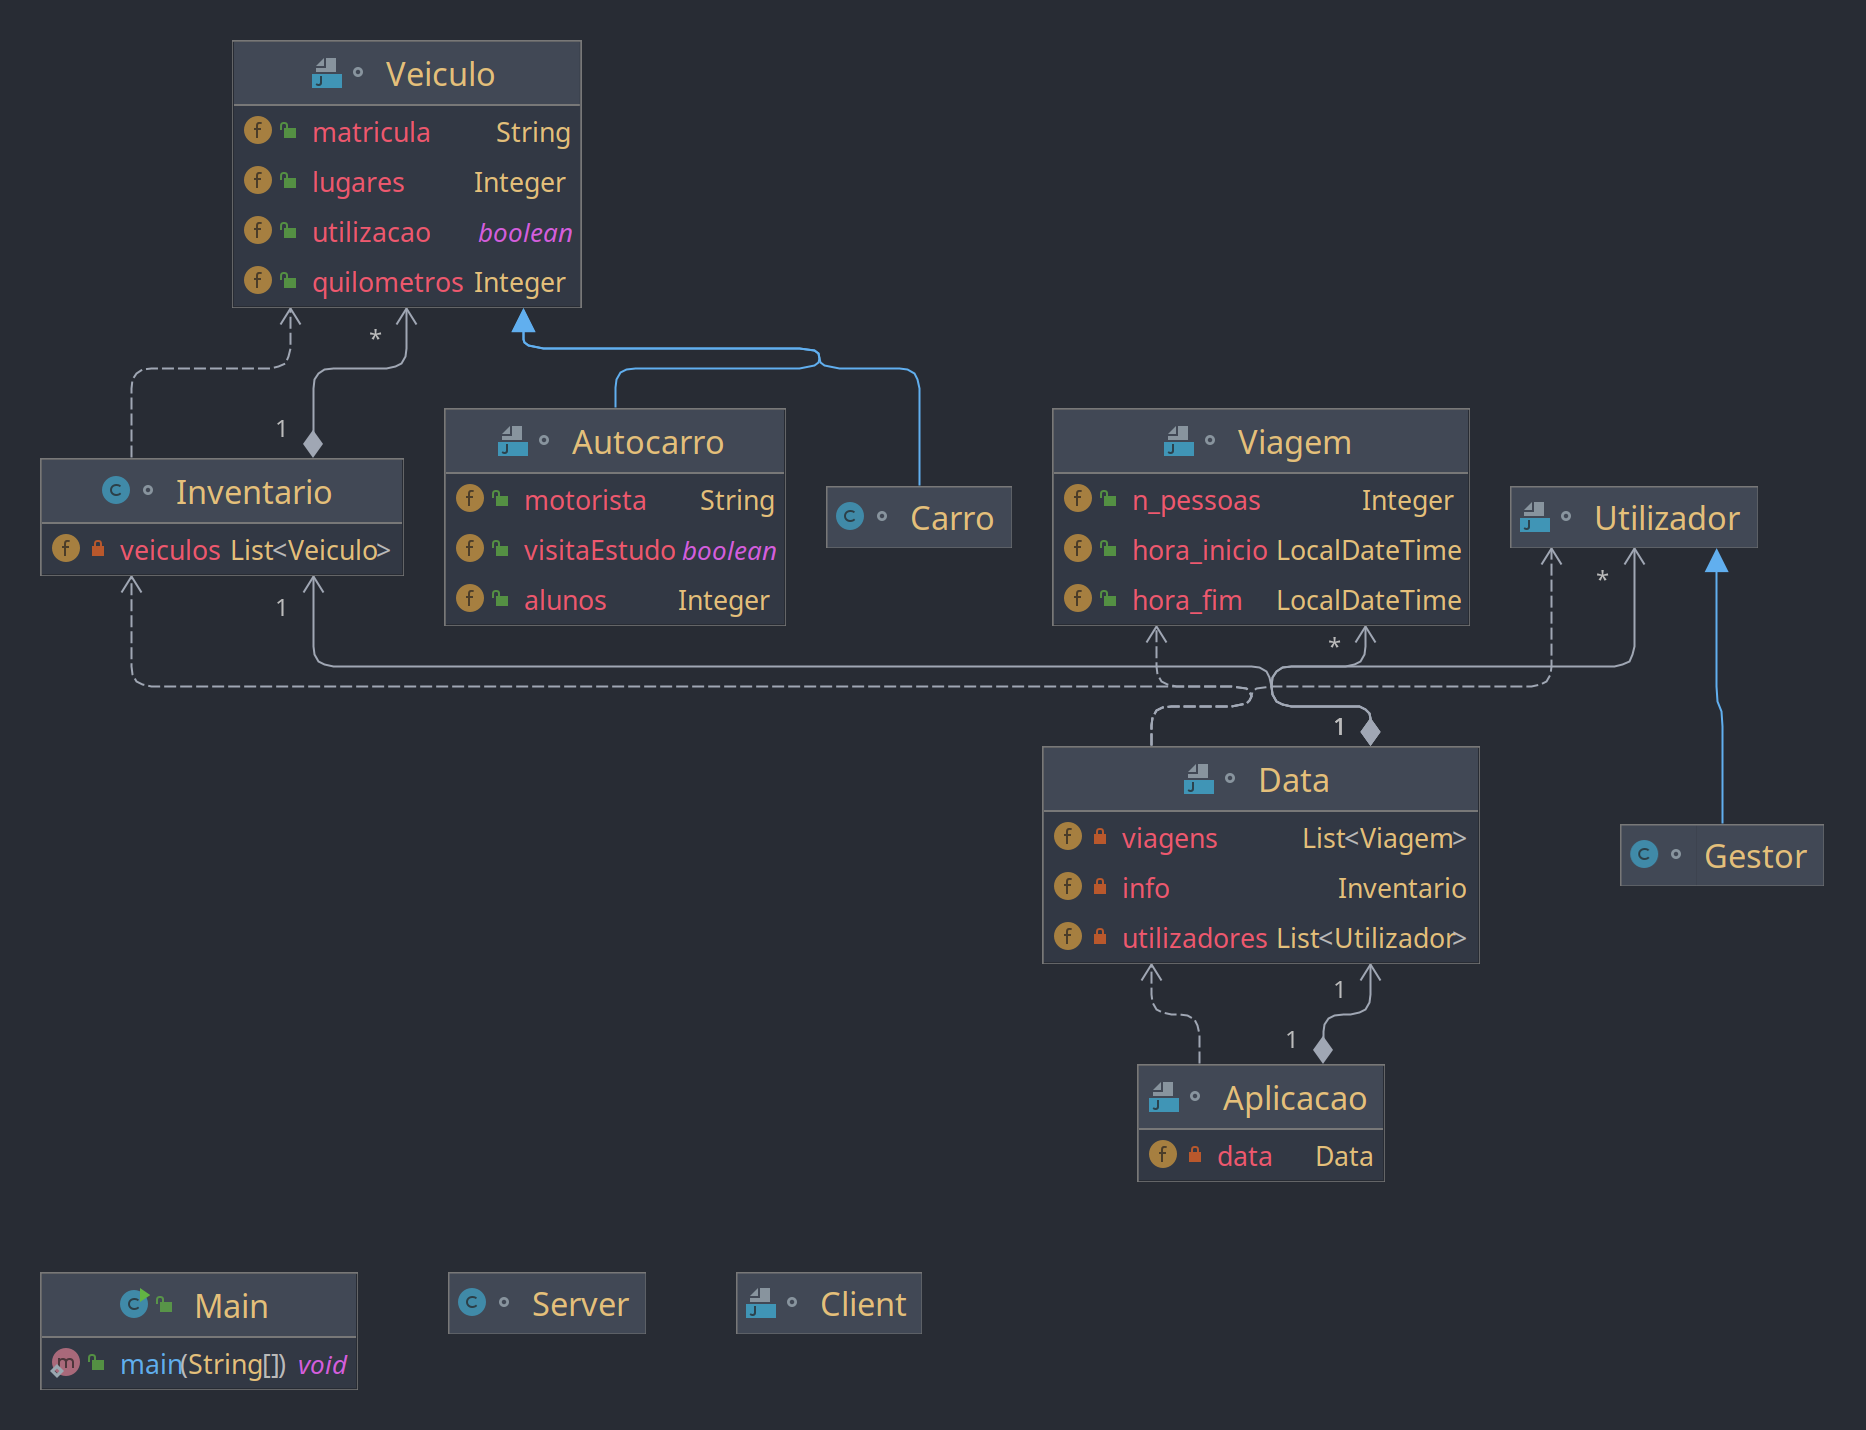
\includegraphics[scale=0.3]{Pictures/Diagrama1.png}
\caption{\label{fig:classes} Diagrama de classes}
\end{figure}







\chapter{Implementação}
\section{O Framework}

Para o desenvolvimento de uma aplicação web, um dos frameworks mais utilizados é o Spring, mais propriamente o Spring boot, que usa o paradigma de desenvolvimento de software "Model-View-Controller" ou "MVC", utilizado em muitas aplicações orientadas aos objetos. Este framework tem ferramentas de "middle-ware", que ajudam a conectar elementos do front-end com o back-end, similares ao javascript. Exemplos de tais ferramentas são as tags "@PostMapping" e "@GetMapping" que quando definidas no html e no java, servem como ponte para passar informação de um extremo da aplicação (interface do utilizador no navegador web) para outro (back-end java e seguidamente mysql). \\
Eis os exemplos destas funcionalidades:\\

\begin{lstlisting}[language=Java, caption=@PostMapping no java]
@PostMapping("/adduser")
    public String addUtilizador(@RequestParam String first, @RequestParam String last, @RequestParam String codigo) {
        Utilizador Utilizador = new Utilizador(first,last,codigo);
        CustomerRepository.save(Utilizador);
        return "Added new Utilizador to repo!";
    }
\end{lstlisting}

No HTML, a tag "action" é mencionada com o valor "/adduser" que está definido no java. É também necessário especificar a tag "method" que especifica se o método é de leitura ou de escrita. Neste exemplo queremos adicionar um utilizador à base de dados, logo no HTML definimos o "form" como "POST" já que queremos escrever na base de dados.

\begin{lstlisting}[language=Html, caption=Método "Post" no Html]
 <form action="/adduser" method="POST" id="user-form">
            <p>Vamos adicionar um utilizador:</p>
            <div>
                <input name="first" id="firstName" type="text" className="form-control" placeholder="Nome próprio" aria-label="Username"
                       aria-describedby="basic-addon1"/>
            </div>
            <div>
                <input name="last" id="lastName" type="text" className="form-control" placeholder="Apelido" aria-label="Username"
                       aria-describedby="basic-addon1"/>
            </div>
            <div>
                <input name="codigo" id="codigo" type="text" className="form-control" placeholder="Codigo" aria-label="Username"
                       aria-describedby="basic-addon1"/>
            </div>
            <br/>
            <div  id="user-button">
                <button type="submit" className="btn btn-outline-primary me-2">Adicionar Utilizador</button>
            </div>
        </form>
\end{lstlisting}

\section{Classes}

Como foi referido anteriormente, o back-end da aplicação tem como suporte as classes "Utilizador", "Veiculo" e "Viagem", definidas no java convencionalmente.\\

\subsection{Utilizador}
Cada elemento da base de dados tem um ID único que é independente do tipo do objeto, ou seja se forem adicionados à base de dados um utilizador, um veículo e uma viagem, estes terão id 1,2 e 3 respetivamente. Este processo é automatizado unicamente pelo Spring, e não é necessário que o programador mantenha um contador dos id's da base de dados. Basta que antes da respetiva variável de instância seja assinalada a tag "@Id" tal como a tag "@Generatedvalue" para que o valor seja incrementado automaticamente.
\begin{lstlisting}[language=Java, caption=Classe Utilizador]
@Entity
public class Utilizador {
    @Id
    @GeneratedValue(strategy = GenerationType.AUTO)
    private Integer id;
    private String nome;
    private String apelido;
    private String codigo; // numero de funcionario
\end{lstlisting}

Estas classes são os objetos mais elementares da aplicação, o agrupar de diferentes utilizadores é registado no "CustomerRepository" definido pelo Spring, e onde podemos definir métodos de procura, entre outros. Este repositório utiliza também as operações CRUD (que foram um dos requisitos mencionados pelos docentes) que serão responsáveis pela manutenção da base de dados e especificam a ligação direta entre o Framework e a base de dados mysql.

\begin{lstlisting}[language=Java, caption=Repositório dos Utilizadores]
public interface CustomerRepository extends CrudRepository<Utilizador, Integer> {
    Utilizador findUtilizadorById(Integer id);
}
\end{lstlisting}

\newpage
\subsection{Veículo}
Da mesma forma que definimos ID's e um repositório para a classe Utilizador, também o fazemos para a classe Veículo. Apresentamos então as variáveis de instância desta classe:

\begin{lstlisting}[language=Java, caption=Classe Veículo]
@Entity
public class Veiculo {
    @Id
    @GeneratedValue(strategy = GenerationType.AUTO)
    private int id;
    private String matricula; // matricula do veiculo
    private int quilometros; // <-- a debater
    private int lugares; // capacidade maxima do veiculo
    private boolean utilizacao; // esta a ser utilizado, mediador de reserva
    private String escola; // escola a que pertence
    private String marca;
    private String modelo;
    private int ano; // ano de fabrico
    private String cor;
    private String combustivel;
    private boolean motorista; // tem ou não motorista
    private String tipo; // tipo do veiculo (carro, autocarro, ...)

\end{lstlisting}

\subsection{Viagem}

\begin{lstlisting}[language=Java, caption=Classe Viagem]
public class Viagem {
    @Id
    @GeneratedValue(strategy = GenerationType.AUTO)
    private int id;
    private Date hora_inicio; // hora do inicio da viagem
    private Date hora_fim; // hora prevista de chegada ao destino
    private String local_de_inicio;
    private String local_de_fim;
    private Integer n_passageiros; // numero de pessoas da viagem ou então uma lista com as pessoas
    private String utilizadores; // lista dos id dos utilizadores
    private int condutor; // ID do utilizador condutor
    private int kms_iniciais;
    private int kms_finais;
    private int veiculo; // ID do veiculo utilizado

\end{lstlisting}

\newpage
\section{Página Web}


Foi implementado uma versão protótipo da aplicação com objetivo de testar os diferentes componentes necessários, como a reserva de viagens da parte de utilizadores, tal como o registo de veículos pela parte de um gestor da aplicação. Optamos por uma abordagem em profundidade, ou seja, disponibilizar todos os campos que necessitam input do utilizador, para que sejam criados os respetivos objetos java, e estes sejam inseridos na base de dados, de modo a  verificar que tudo funciona corretamente. Podemos assim, na fase de desenvolvimento estético da aplicação, reorganizar apenas estes campos na página web.

\begin{figure}[h!]
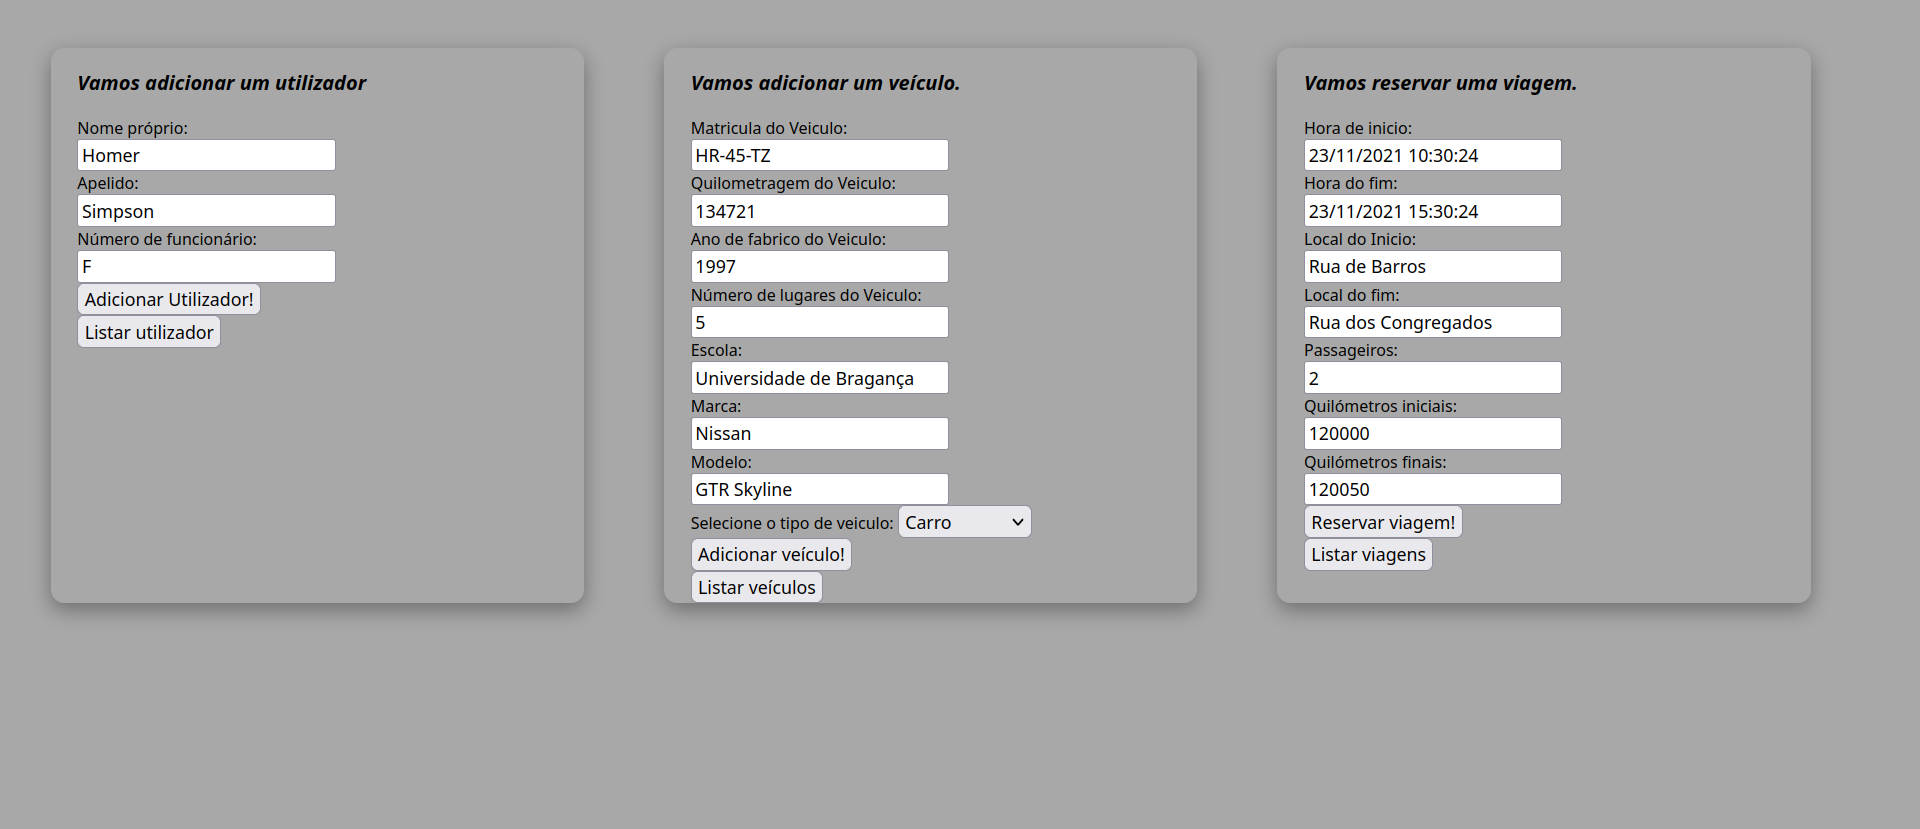
\includegraphics[scale=0.35]{Pictures/localhost.png}
\caption{\label{fig:html} Prótótipo do website desenvolvido em html.}
\end{figure}

O Spring é flexível e é possível integrar varias "Views" e frameworks que melhor se adaptam às necessidades do desenvolvimento web comtemporaneo. 
Com o pacote "create-react-app" podemos configurar um ambiente de trabalho dentro do Spring que substitui a view tradicional que este usa, e nos deixa desenhar um website muito mais responsivo.
\pageref{bib}

\begin{figure}[h!]
\centering
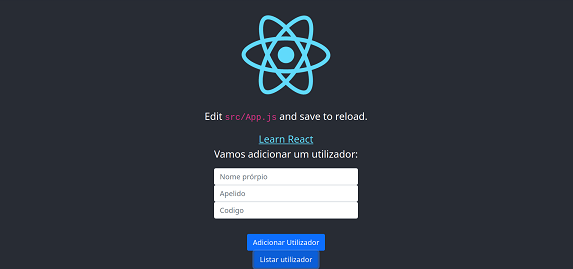
\includegraphics[scale=1.0]{Pictures/Menu1.png}
\caption{\label{fig:Diagrama} Página Web Temporária}
\end{figure}

Após algum desenvolvimento da página web em React desenvolvemos um layout mais amigável ao utilizador. No React, os componentes são os "tijolos" que constroem a página web. Na nossa aplicação, "App" é o componente principal, e o que trata do redirecionamento para diferentes páginas dentro do site. Está definido da seguinte forma:  

\begin{lstlisting}[language=Html, caption=Componente App do React]
function App() {
    return (
        <Router>
            <div className="App">
                <Routes>
                    <Route exact path="/" element={<Home/>}/>
                    <Route path="/veiculos" element={<Veiculos/>}/>
                </Routes>
            </div>
        </Router>
    );
}
\end{lstlisting}

Utilizamos o pacote "react-router-dom" que pode ser facilmente incluido em qualquer aplicação React com o comando:
\begin{lstlisting}[language=bash]
  $ npm install react-router-dom
\end{lstlisting}
Este é o pacote mais utilizado por desenvolvedores de aplicações web em React para redirecionamento. \\
O próximo componente do site é "Home", que decora a página inicial com uma barra de navegação e um menu para input do utilizador. Mais tarde serão desenvolvidas as funcionalidades de registo de log-in de utilizadores, mas para já os respetivos botões já se encontram na nav-bar. 
Existem tags "Link" no código fonte da página inicial que pertencem ao pacote react-router-dom, que se encarregam de especificar o novo endereço do website caso ocorra um clique nas abas de "Registo", "Veiculo", etc. \\


Para uma customização mais profunda do aspeto da página web, foi utilizada a biblioteca "Bootstrap", que tem componentes pré-definidos como botões e menus, que para além de facilitar o desenvolvimento, dão um aspeto profissional à página. 
\begin{figure}[h!]
\centering
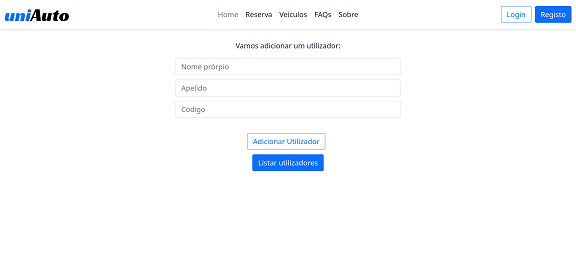
\includegraphics[scale=1.0]{Pictures/Menu3.png}
\caption{\label{fig:Diagrama} Página Atualizada}
\end{figure}
\newpage

\section{Alternativas, Decisões e Problemas de Implementação}

\begin{figure}[h!]
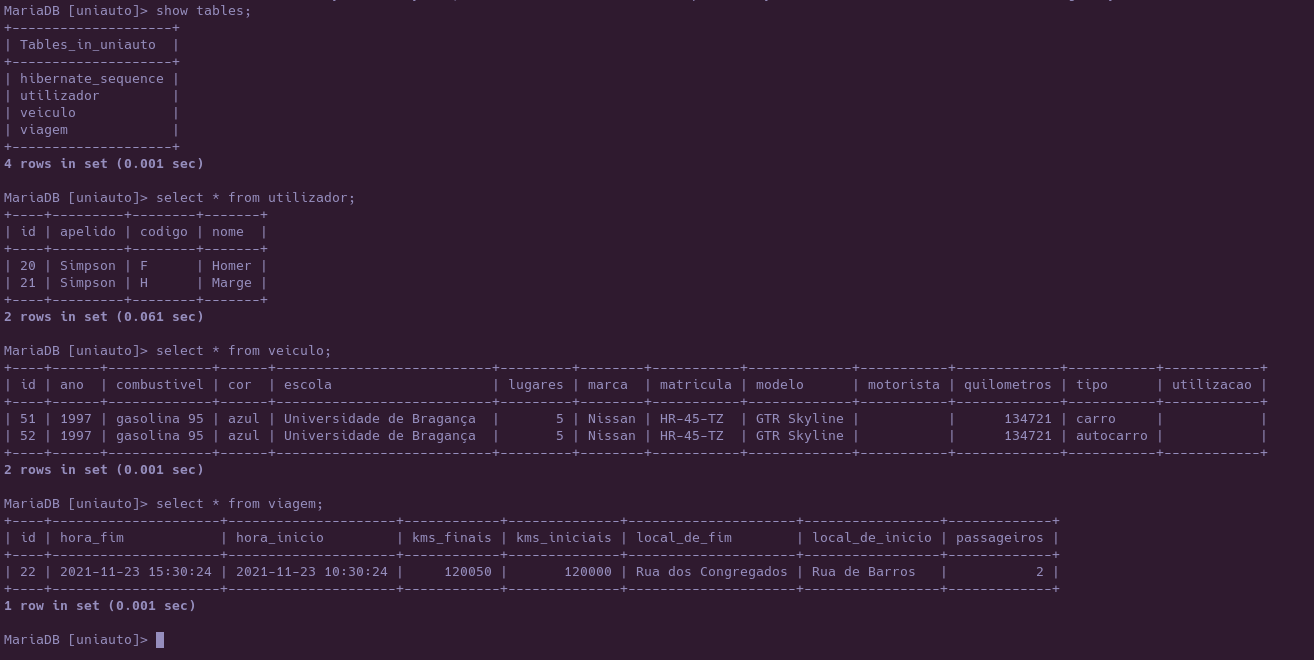
\includegraphics[scale=0.5]{Pictures/db.png}
\caption{\label{fig:Mysql} Exemplo primitivo da configuração da base de dados no mysql.}
\end{figure}
\newpage




\section{Testes Realizados e Resultados}
%"mystyle" code listing set
\lstset{style=mystyle}

\begin{lstlisting}[language=Java, caption=Teste em java]
@SpringBootTest
class UniAutoApplicationTests {

    @Test
    public void whenCustomSerializingAndDeserializing_ThenObjectIsTheSame()
            throws IOException, ClassNotFoundException {
        Person p = new Person();
        p.setAge(20);
        p.setName("Joe");


        FileOutputStream fileOutputStream
                = new FileOutputStream("yourfile2.txt");
        ObjectOutputStream objectOutputStream
                = new ObjectOutputStream(fileOutputStream);
        objectOutputStream.writeObject(p);
        objectOutputStream.flush();
        objectOutputStream.close();

        FileInputStream fileInputStream
                = new FileInputStream("yourfile2.txt");
        ObjectInputStream objectInputStream
                = new ObjectInputStream(fileInputStream);
        Person p2 = (Person) objectInputStream.readObject();
        objectInputStream.close();

/*
        System.out.println("p nome: "+p.getName());
        System.out.println("p idade: "+p.getAge());
        System.out.println("p2 nome: "+p2.getName());
        System.out.println("p2 idade: "+p2.getAge());
*/
        assertTrue(
                p2.getName().equals( p.getName()));
        assertTrue(
                Objects.equals(p2.getAge(), p.getAge()));
    }
}
\end{lstlisting}
\newpage
\chapter{Manual de Utilização}
\section{Adicionar Utilizador}

\begin{figure}[h!]
\centering
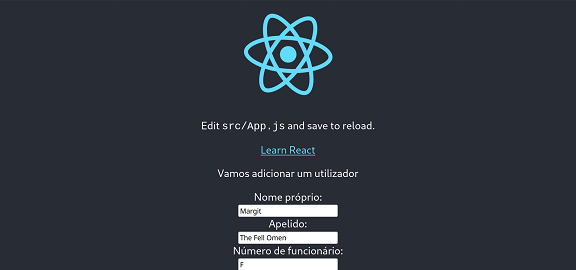
\includegraphics[scale=1.0]{Pictures/reactToBD.png}
\caption{\label{fig:Diagrama} Adicionar Utilizador através do React}
\end{figure}

\begin{figure}[h!]
\centering
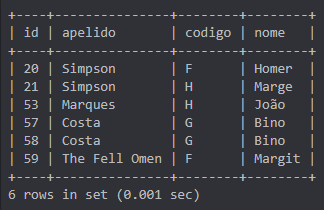
\includegraphics[scale=1.6]{Pictures/InserçãoBD.png}
\caption{\label{fig:Diagrama} Utilizador Adicionado com sucesso à BD}
\end{figure}

\cite{*} %zau
\bibliographystyle{alpha}

\bibliography{refs}

\end{document}